% Compile: pdfLaTeX (or LuaLaTeX). Overleaf-friendly.
% Focused deck: hipVS (RDNA3 warp32) vs cuVS library speed on peer GPUs.
\documentclass[aspectratio=169,11pt]{beamer}

\usetheme{Madrid}
\usecolortheme{whale}
\setbeamertemplate{navigation symbols}{}
\setbeamertemplate{footline}[frame number]
\setbeamerfont{title}{size=\Large\bfseries}
\setbeamerfont{frametitle}{size=\large\bfseries}

\usepackage{booktabs}
\usepackage{tikz}
\usepackage{pgfplots}
\pgfplotsset{compat=1.18}

\title{hipVS vs cuVS --- Library Speed}
\subtitle{RDNA3 (\texttt{warp\_size}=32) on RX~7900~XTX vs RTX~4080}
\author{Konstantin Kolchin}
\date{23 July 2026}

\begin{document}

%----- title -----
\begin{frame}
  \titlepage
  \vspace{0.3em}
  \begin{center}
    \small
    Direct library API (no Milvus).\\
    Same recipe, peer GPUs --- not identical silicon.
  \end{center}
\end{frame}

%----- ask -----
\begin{frame}{The question}
  \begin{block}{Context}
    hipVS runs on RDNA3 with \texttt{warp\_size}=32
    (\texttt{USE\_WARPSIZE\_32}).\\
    Does that library keep up with NVIDIA cuVS?
  \end{block}

  \vspace{0.6em}
  \textbf{What this deck shows}
  \begin{itemize}
    \item Same Python API: \texttt{import cuvs} (hipVS keeps the name)
    \item Same workload on both GPUs
    \item \textbf{Answer quality} (recall@10) and \textbf{throughput} (QPS)
  \end{itemize}

  \vspace{0.5em}
  {\footnotesize Not a product-path speed claim --- SIFT Milvus is stack-limited
  (see later slides). Fair Milvus NVIDIA-ahead hunt: GIST PQ.}
\end{frame}

%----- setup -----
\begin{frame}{Measurement setup}
  \footnotesize
  \begin{center}
  \begin{tabular}{@{}ll@{}}
    \toprule
    \textbf{Field} & \textbf{Freeze} \\
    \midrule
    API & Python \texttt{cuvs.neighbors} (no Milvus / Knowhere) \\
    Dataset & SIFT-1M (\texttt{sift-128-euclidean.hdf5}) \\
    Index & IVF\_PQ, $m{=}32$, $nbits{=}8$, $nlist{=}1024$ \\
    Search & $k{=}10$; \texttt{nprobe} $\in \{1,4,8,16,32\}$ \\
    AMD & RX 7900 XTX --- hipVS (ROCm, warp~32) \\
    NVIDIA & RTX 4080 --- cuVS (CUDA) \\
    Metric & Batched QPS; recall@10 vs HDF5 ground truth \\
    \bottomrule
  \end{tabular}
  \end{center}

  \vspace{0.5em}
  \begin{block}{Fairness}
    Same code path / recipe. GPUs are \textbf{peer-class}, not the same chip.\\
    Speed-up $=$ hipVS QPS $/$ cuVS QPS.
  \end{block}
\end{frame}

%----- headline -----
\begin{frame}{Headline result}
  \begin{columns}[T]
    \begin{column}{0.48\textwidth}
      \begin{block}{Quality}
        \centering\large
        Recall@10 \textbf{matches}\\[0.3em]
        {\normalsize $0.35 \rightarrow 0.72$}\\[0.2em]
        {\footnotesize (same on both GPUs)}
      \end{block}
    \end{column}
    \begin{column}{0.48\textwidth}
      \begin{block}{Speed}
        \centering\large
        hipVS $\approx$ \textbf{0.5$\times$} cuVS\\[0.3em]
        {\normalsize QPS ratio $0.37$--$0.55\times$}\\[0.2em]
        {\footnotesize across the nprobe grid}
      \end{block}
    \end{column}
  \end{columns}

  \vspace{0.8em}
  \begin{center}
    \Large
    Same answers; \textbf{ratio depends on the index}.\\[0.25em]
    {\normalsize IVF\_PQ $m{=}32$: cuVS $\sim$2$\times$ hipVS.\\
     IVF\_FLAT high-\texttt{nprobe}: hipVS $\sim$1.3$\times$ cuVS.}
  \end{center}
\end{frame}

%----- table -----
\begin{frame}{QPS and recall by nprobe}
  \footnotesize
  Direct \texttt{cuvs} API --- IVF\_PQ ($m{=}32$).\\[0.35em]

  \begin{center}
  \begin{tabular}{@{}lrrrrr@{}}
    \toprule
    \textbf{nprobe}
      & \textbf{hipVS QPS} & \textbf{cuVS QPS}
      & \textbf{R@10} & \textbf{hip/cu} & \textbf{cu/hip} \\
    \midrule
    1  & 1.59M & 4.33M & 0.35 & $0.37\times$ & $2.71\times$ \\
    4  & 1.27M & 2.30M & 0.59 & $0.55\times$ & $1.81\times$ \\
    8  & 0.71M & 1.41M & 0.67 & $0.50\times$ & $1.99\times$ \\
    16 & 0.39M & 0.81M & 0.71 & $0.49\times$ & $2.05\times$ \\
    32 & 0.22M & 0.45M & 0.72 & $0.48\times$ & $2.09\times$ \\
    \bottomrule
  \end{tabular}
  \end{center}

  \vspace{0.45em}
  {\footnotesize
  Sources: \texttt{lib\_hipvs\_ivf\_pq\_m32\_20260723\_211759.json},
  \texttt{lib\_cuvs\_ivf\_pq\_m32\_20260723\_201837.json}.}
\end{frame}

%----- heavy FLAT -----
\begin{frame}{GPU-heavy library --- IVF\_FLAT (high nprobe)}
  \footnotesize
  Same API / SIFT-1M / \texttt{nlist}=1024.
  Higher \texttt{nprobe} $\Rightarrow$ more GPU work (QPS halves when \texttt{nprobe} doubles).\\[0.3em]

  \begin{center}
  \begin{tabular}{@{}lrrrr@{}}
    \toprule
    \textbf{nprobe}
      & \textbf{hipVS QPS} & \textbf{cuVS QPS}
      & \textbf{R@10} & \textbf{hip/cu} \\
    \midrule
    32  & 64142 & 49039 & 0.978 & $1.31\times$ \\
    64  & 33381 & 24759 & 0.996 & $1.35\times$ \\
    128 & 17200 & 12498 & 0.999 & $1.38\times$ \\
    256 & 8784  & 6332  & 0.999 & $1.39\times$ \\
    \bottomrule
  \end{tabular}
  \end{center}

  \vspace{0.4em}
  \textbf{Takeaway:} on this compute-bound FLAT load, AMD~7900 is
  \textbf{$\sim$1.3--1.4$\times$} the 4080 (peer GPUs).\\
  {\footnotesize Contrast PQ table ($\sim$0.5$\times$). Kernel mix matters.
  Sources: \texttt{results/lib\_bench/FILLED\_flat\_heavy.md}.}
\end{frame}

%----- QPS plot -----
\begin{frame}{QPS --- hipVS vs cuVS (IVF\_PQ $m=32$)}
  \vspace{-0.2em}
  {\footnotesize Batched search. Higher is faster.
  {\color{red}AMD~7900} / {\color{green!60!black}NVIDIA~4080}.}\\[0.1em]
  \centering
  \begin{tikzpicture}
    \begin{axis}[
      width=0.95\textwidth,
      height=0.62\textheight,
      xlabel={nprobe},
      ylabel={QPS},
      xmin=0, xmax=34,
      ymin=0, ymax=5.0e6,
      xtick={1,4,8,16,32},
      legend style={at={(0.98,0.98)},anchor=north east,font=\small},
      grid=major,
      major grid style={gray!30},
    ]
      \addplot[thick,red,mark=*,mark size=2.5pt] coordinates {
        (1,1593707) (4,1268942) (8,710989) (16,393742) (32,217275)
      };
      \addlegendentry{AMD hipVS (7900 XTX)}
      \addplot[thick,green!60!black,mark=square*,mark size=2.5pt] coordinates {
        (1,4326105) (4,2297667) (8,1411722) (16,806267) (32,453316)
      };
      \addlegendentry{NVIDIA cuVS (RTX 4080)}
    \end{axis}
  \end{tikzpicture}
\end{frame}

%----- ratio plot -----
\begin{frame}{Speed-up ratio (hipVS / cuVS)}
  \vspace{-0.2em}
  {\footnotesize $1.0$ $=$ parity. Measured band $\approx 0.37$--$0.55$.}\\[0.1em]
  \centering
  \begin{tikzpicture}
    \begin{axis}[
      width=0.95\textwidth,
      height=0.60\textheight,
      xlabel={nprobe},
      ylabel={Speed-up (hip / cu)},
      xmin=0, xmax=34,
      ymin=0, ymax=1.2,
      xtick={1,4,8,16,32},
      ytick={0,0.25,0.5,0.75,1.0},
      grid=major,
      major grid style={gray!30},
    ]
      \addplot[thick,red,mark=*,mark size=2.5pt] coordinates {
        (1,0.368) (4,0.552) (8,0.504) (16,0.488) (32,0.479)
      };
      \addplot[dashed,gray,thick] coordinates {(0,1) (34,1)};
      \node[anchor=west,gray,font=\small] at (axis cs:20,1.05) {parity};
      \addplot[dashed,red!50!black] coordinates {(0,0.5) (34,0.5)};
      \node[anchor=west,red!50!black,font=\small] at (axis cs:20,0.55) {$\sim$0.5$\times$};
    \end{axis}
  \end{tikzpicture}
\end{frame}

%----- recall -----
\begin{frame}{Recall@10 --- same on both}
  \vspace{-0.2em}
  {\footnotesize Curves overlap ($\Delta{<}0.002$). Markers: filled~{\color{red}AMD}, open~{\color{green!60!black}NVIDIA}.}\\[0.1em]
  \centering
  \begin{tikzpicture}
    \begin{axis}[
      width=0.95\textwidth,
      height=0.58\textheight,
      xlabel={nprobe},
      ylabel={recall@10},
      xmin=0, xmax=34,
      ymin=0.2, ymax=0.85,
      xtick={1,4,8,16,32},
      legend style={at={(0.98,0.3)},anchor=south east,font=\small},
      grid=major,
      major grid style={gray!30},
    ]
      % Draw NVIDIA first (under), AMD on top --- values match within noise
      \addplot[
        thick,dashed,green!60!black,
        mark=square*,
        mark size=3.2pt,
        mark options={solid,fill=white,draw=green!60!black},
      ] coordinates {
        (1,0.3463) (4,0.5911) (8,0.6673) (16,0.7085) (32,0.7249)
      };
      \addlegendentry{NVIDIA cuVS}
      \addplot[
        thick,red,
        mark=*,
        mark size=2.2pt,
      ] coordinates {
        (1,0.3477) (4,0.5918) (8,0.6672) (16,0.7086) (32,0.7247)
      };
      \addlegendentry{AMD hipVS}
    \end{axis}
  \end{tikzpicture}
\end{frame}

%----- library vs milvus -----
\begin{frame}{SIFT Milvus is stack-limited (not a speed verdict)}
  \footnotesize
  Same peer GPUs, IVF\_PQ $m{=}32$. \textbf{Library} $=$ direct \texttt{cuvs} API;
  \textbf{Milvus} $=$ product path (RPC + Knowhere).\\[0.3em]

  \begin{center}
  \begin{tabular}{@{}llrrrr@{}}
    \toprule
    \textbf{Path} & \textbf{nprobe}
      & \textbf{{\color{red}AMD} QPS} & \textbf{{\color{green!60!black}NVIDIA} QPS}
      & \textbf{AMD/NVIDIA} & \textbf{Scale} \\
    \midrule
    Library & 8  & 0.71M & 1.41M & $0.50\times$ & --- \\
    Library & 32 & 0.22M & 0.45M & $0.48\times$ & --- \\
    \midrule
    Milvus SIFT & 8  & 19500 & 19786 & $0.99\times$ & $\sim$36$\times$ below lib \\
    Milvus SIFT & 32 & 14784 & 14144 & $1.05\times$ & $\sim$15$\times$ below lib \\
    \bottomrule
  \end{tabular}
  \end{center}

  \vspace{0.35em}
  {\scriptsize
  ``Scale'' $=$ how much lower Milvus QPS is than library QPS (AMD column).
  SIFT product path hides the library gap --- do \textbf{not} call this
  ``AMD competitive on ANN.''}\\[0.25em]

  \begin{columns}[T]
    \begin{column}{0.48\textwidth}
      \begin{block}{Library}
        \footnotesize
        Kernels dominate.\\
        hipVS $\sim$0.5$\times$ cuVS (PQ).\\
        QPS in the $10^5$--$10^6$ range.
      \end{block}
    \end{column}
    \begin{column}{0.48\textwidth}
      \begin{block}{Milvus SIFT}
        \footnotesize
        RPC / stack dominate.\\
        Ratio $\sim$1$\times$ is expected.\\
        Need GPU-heavy recipe next.
      \end{block}
    \end{column}
  \end{columns}
\end{frame}

%----- product contrast -----
\begin{frame}{SIFT product path --- recall OK, speed inconclusive}
  \footnotesize
  Batched SIFT-1M Milvus (Knowhere + RPC). Speed-up $=$ AMD QPS / CUDA QPS.\\
  Valid for \textbf{port correctness}; \textbf{not} for ``who is faster at ANN.''\\[0.35em]

  \begin{center}
  \begin{tabular}{@{}llrrr@{}}
    \toprule
    \textbf{Index} & \textbf{nprobe}
      & \textbf{{\color{red}AMD} QPS} & \textbf{{\color{green!60!black}CUDA} QPS} & \textbf{Speed-up} \\
    \midrule
    IVF\_FLAT & 8  & 21838 & 19800 & $1.10\times$ \\
    IVF\_FLAT & 32 & 19578 & 13868 & $1.41\times$ \\
    IVF\_PQ $m{=}32$ & 8  & 19500 & 19786 & $0.99\times$ \\
    IVF\_PQ $m{=}32$ & 32 & 14784 & 14144 & $1.05\times$ \\
    \bottomrule
  \end{tabular}
  \end{center}

  \vspace{0.5em}
  \begin{block}{Fair Milvus speed --- GIST-1M \texttt{GPU\_IVF\_PQ} $m{=}32$ (2026-07-28)}
    \footnotesize
    \begin{center}
    \begin{tabular}{@{}lrrr@{}}
      \toprule
      \textbf{nprobe}
        & \textbf{{\color{red}AMD} QPS}
        & \textbf{{\color{green!60!black}CUDA} QPS}
        & \textbf{AMD/CUDA} \\
      \midrule
      8   & 4867 & 7167 & $0.68\times$ \\
      16  & 2945 & 4102 & $0.72\times$ \\
      32  & 2228 & 2774 & $0.80\times$ \\
      64  & 1145 & 1908 & $0.60\times$ \\
      128 & 700  & 959  & $0.73\times$ \\
      \bottomrule
    \end{tabular}
    \end{center}
    Recall@10 matches ($\sim$0.25--0.27). NVIDIA ahead;
    runbook: \texttt{docs/milvus\_amd\_behind\_nvidia\_plan.md}.
  \end{block}
\end{frame}

%----- takeaway -----
\begin{frame}{Takeaway for management}
  \begin{enumerate}
    \item \textbf{RDNA3 hipVS works} (\texttt{warp\_size}=32) --- answers match cuVS.
    \item \textbf{Raw library:} ratio is kernel-dependent ---
          IVF\_PQ $m{=}32$ $\sim$0.5$\times$; IVF\_FLAT high-\texttt{nprobe} $\sim$1.3$\times$.
    \item \textbf{Milvus:} SIFT is stack-limited ($\sim$1$\times$);
          \textbf{GIST PQ} shows NVIDIA ahead (AMD/CUDA $\sim$0.60--0.80$\times$).
  \end{enumerate}

  \vspace{0.6em}
  \begin{center}
    \large
    Correct port. Library PQ gap is real.\\[0.15em]
    Under GPU-heavy Milvus, AMD trails --- fair product signal.
  \end{center}

  \vspace{0.5em}
  {\footnotesize
  Lab 2026-07-23/27 (lib) / 2026-07-28 (Milvus GIST).
  \texttt{results/milvus\_gist\_pq/FILLED.md}.}
\end{frame}

\end{document}
